\RequirePackage{ifluatex}
\let\ifluatex\relax

\documentclass[aps,%
12pt,%
final,%
oneside,
onecolumn,%
musixtex, %
superscriptaddress,%
centertags]{article} %% 
\topmargin=-40pt
\textheight=650pt
\usepackage[english,russian]{babel}
\usepackage[utf8]{inputenc}
%всякие настройки по желанию%
\usepackage[colorlinks=true,linkcolor=black,unicode=true]{hyperref}
\usepackage{euscript}
\usepackage{supertabular}
\usepackage[pdftex]{graphicx}
\usepackage{amsthm,amssymb, amsmath}
\usepackage{textcomp}
\usepackage[noend]{algorithmic}
\usepackage[ruled]{algorithm}
\usepackage{lipsum}
\usepackage{indentfirst}
\usepackage{babel}
\usepackage{pgfplots}
\pgfplotsset{compat=1.9}

\pgfplotsset{model/.style = {blue, samples = 100}}
\pgfplotsset{experiment/.style = {red}}

\selectlanguage{russian}

\setlength{\parindent}{2.4em}
\setlength{\parskip}{0.1em}
%\renewcommand{\baselinestretch}{2.0}

\usepackage{xcolor}
\usepackage{hyperref}
 
 % Цвета для гиперссылок
%\definecolor{linkcolor}{HTML}{799B03} % цвет ссылок
%\definecolor{urlcolor}{HTML}{799B03} % цвет гиперссылок
 
%\hypersetup{pdfstartview=FitH,  linkcolor=linkcolor,urlcolor=urlcolor, colorlinks=true}

%\documentclass[aps,%
%12pt,%
%final,%
%oneside,
%onecolumn,%
%musixtex, %
%superscriptaddress,%
%centertags]{article} %% 
%\topmargin=-40pt
%\textheight=650pt
%\usepackage[english,russian]{babel}
%\usepackage[utf8]{inputenc}
%всякие настройки по желанию%
%\usepackage[colorlinks=true,linkcolor=blue,unicode=true]{hyperref}
%\usepackage{euscript}
%\usepackage{supertabular}
%\usepackage[pdftex]{graphicx}
%\usepackage{amsthm,amssymb, amsmath}
%\usepackage{textcomp}
%\usepackage[noend]{algorithmic}
%\usepackage[ruled]{algorithm}
%\selectlanguage{russian}

\begin{document}

\begin{titlepage} 
\begin{center}
% Upper part of the page
%\textbf{\Large САНКТ-ПЕТЕРБУРГСКИЙ ГОСУДАРСТВЕННЫЙ ЭКОНОМИЧЕСКИЙ УНИВЕРСИТЕТ} \\[1.0cm]
%\textbf{\large Кафедра Прикладной Математики и Информатики}\\[3.5cm]
 
% Title
\textbf{}\\[10.0cm]
\textbf{\LARGE Финансовая математика}\\[0.5cm]
\textbf{\Large ПМ-1701} \\[0.2cm]

%supervisor
\begin{center} \large
{Преподаватель:} \\[0.5cm]
\textsc {Чернов Алексей Викторович}\\
{alex\_tche@mail.ru}\\
\end{center}
% \begin{flushright} \large
%\emph{Рецензент:} \\
%д.ф. - м.н., профессор \textsc{Надеемся Нам Помогут}
%\end{flushright}
%\begin{flushright} \large
%\emph{Заведующий кафедрой:} \\
%д.ф. - м.н., профессор \textsc{Не Обмани Себя}
%\end{flushright}
\vfill 

% Bottom of the page
{\large {Санкт-Петербург}} \par
{\large {2020 г., 6 семестр}}
\end{center} 
\end{titlepage}

% Table of contents
\begin{thebibliography}{3}
	\bibitem{Sulsky1994}
	Sulsky D., Chen Z., Schreyer H. L.  A particle method for history-dependent materials // Computer Methods in Applied Mechanics and Engineering. --- 1994, V. 118. --- P. 179--196.
	\bibitem{LiuLiu}
	Liu G. R., Liu M. B. Smoothed particle hydrodynamics: a meshfree particle method. --- Singapore : World Scientific Publishing. --- 2003. --- 449 p.
\end{thebibliography}
\tableofcontents
\newpage
\section{Конспекты лекций}
\subsection{ Простая и сложная процентная ставка 05.02.2020} 

Для иллюстрации понимания работы сложного и простого процента введем следующие обозначения:
\begin{itemize} 
  \item $i$ - процентная ставка (по умолчанию годовая)
  \item $t$ - срок вклада
  \item $S_{0} = P$ - начальный вклад
  \item \textbf{$S$} - конечный вклад
  
\end{itemize}

Опр: \textit{Простыми процентами} называются такие процентные ставки, которые применяются к одной и той же первоначальной сумме на протяжении всей финансовой операции

Опр: \textit{Сложными процентами} называются ставки, применяемые после каждого интервала начисления к сумме первоначального долга и начисленных за предыдущие интервалы процентов.
\label{first_table}
\begin{table}[H]
	\begin{center}
		\begin{tabular}{c|c|c} 
		t (год) & Простой процент (\%) & Сложный процент (\%) \\ \hline
		0 & \textbf{100} & 100  \\ 
		1 & \textbf{110} & 110 \\ 
		2 & \textbf{120} & 121
		\end{tabular}
	\caption{Пример использования сложных и простых процентов}
	\end{center}
\end{table}
\subsubsection{Формулы простых процентов}
Формула для $S_{n+1}$: $$S_{n+1}=S_n+S_0\cdot i  $$

Формула для конечного вклада: $$S=P+P\cdot i\cdot n=P\cdot (1+i\cdot n) $$

Формула для начального вклада: $$P=\frac{S}{1+i\cdot n} $$

Формула для процентной ставки: $$i=\frac{\frac{S}{P}-1}{t}=\frac{S-P}{t\cdot P}$$

Формула для продолжительности вклада: $$ t=\frac{\frac{S}{P}-1}{i}=\frac{S-P}{i\cdot P}$$

\subsubsection{Формулы простых процентов}
Формула для $S_{n+1}$: $$S_{n+1}=S_n\cdot (1+i) = S_n + S_n\cdot i  $$

Формула для конечного вклада: $$S = P\cdot (1+i)^n $$

Формула для начального вклада: $$P=\frac{S}{(1+i)^n} $$

Формула для процентной ставки: $$i=\sqrt[t]{\frac{S}{P}}-1$$

Формула для продолжительности вклада: $$ t=log_{(1+i)} \frac{S}{P}$$

\subsubsection{Срок удвоения вклада}

\textbf {Для простого процента:} 
$$2P=P\cdot(1+i\cdot t_{new})$$ 
$$t_{new}=\frac{1}{i}$$

\textbf {Для сложного процента:} 
$$2P=P\cdot(1+i)^{t_{new}}$$ 
$$2 = (1+i)^{t_{new}}$$ 
$$t_{new}=log_{(1+i)} 2 $$

\subsubsection{Задача о.в Манхэттен}
\label{second_table}
\begin{table}[H]
	\begin{center}
		\begin{tabular}{c|c} 
		t (год) & Деньги (\$) \\ \hline
		$t_1$ - 1626 год & $P - 24$ \\ \hline
		$t_2$ - 2019 год & $S - 49\cdot 10^9$
		\end{tabular}
		\caption{Данные о Манхэттене}
	\end{center}
\end{table}

\textbf{Вопрос}: Какова процентная ставка при простом и сложном проценте?

\textbf{Решение:}

Простой процент: 
$$i=\frac{\frac{S}{P}-1}{t}=\frac{S-P}{(t_2-t_1)\cdot P}=\frac{49\cdot 10^9-24}{24*(2019-1626)}=5.19 \cdot 10^6$$

Сложный процент: 
$$i=\sqrt[(t_2-t_1)]{\frac{S}{P}}-1=\sqrt[2019-1626]{\frac{49\cdot 10^9}{24}}-1 = 0.056 = 5.6\%$$

Срок удвоения оклада: 
$$t_{new}=log_{(1+i)} 2 = log_{(1+0.056)} 2 = 12.7 \approx 13 \text{ years}$$ 

\subsubsection{Смешанная ставка}

Опр: \textit{Смешанная процентная ставка} - ставка, которая осуществляется по следующему правилу - в пределах года используется простая ставка, а остальные - по сложной.

Формула для смешанной процентной ставки:
$$S = P\cdot (1+i_c)^{[t]} + P\cdot (1+i_c)^{[t]} \cdot {\{t\}}\cdot i_p = P(1+i_c)^{[t]} \cdot (1 + {\{t\}}\cdot i_p ) $$
где ${[t]}$ - целая часть числа, а  ${\{t\}}$ - дробная.
\begin{figure}[h!]
	
	\begin{center}
	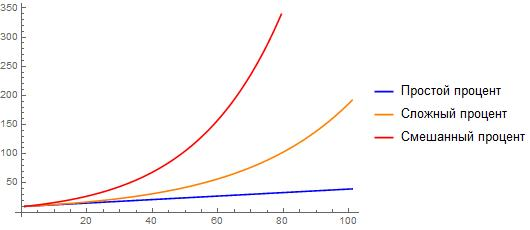
\includegraphics[scale=0.6]{images/first.jpg}
	\caption{График простой, сложной и процентной ставки}
	\end{center}
\end{figure}
\newpage


\subsection{Процентная ставка для разных периодов времени 09.02.2020 }

Пусть задана простая процентная ставка. Нужно найти эквивалентную месячную ставку.
$$ P\cdot (1+i_{year} \cdot t) = P \cdot (1+12 \cdot i_{m}\cdot t) $$
$$i_{m} = \frac{i_{year}}{12} $$
$$i_{d} = \frac{i_{year}}{365} $$

Такой способ приведения и соотношения называются \textit{относительными}.

Для сложных процентов:
$$ S = P\cdot (1+i_{year})^n  = P\cdot (1+i_{m})^{12n} $$
$$ i_{m} = \sqrt[12]{1 + i_{year}} - 1 $$

А такой способ называется \textit{уравновешенным}.

Пример:

Банк предъявляет простую годовую ставку $i_{year}$ на срок до $3$-х лет. Можем ли мы придумать более легкую стратегию? Да, мы можем положить деньги на вклад, снять деньги, а потом заново открыть вклад. Рассмотрим решение задачи двумя разными способами:

\textbf{Решение:}

$$ P \cdot (1+i \cdot t) < P (1+i)^t $$

Если использовать месячную ставку, то получаем формулу:

$$(1+\frac{i}{12})^{12} = {Binom Newion} = 1 + 12 \frac{i}{12} + ... + > (1+i) $$
$$ i>0 \text{, } t > 1 $$
$$ \lim_{m\to \infty} (1+\frac{i}{m})^{t\cdot m} = \lim_{m\to \infty} ((1+\frac{i}{m})^{\frac{m}{i}})^{t\cdot i} = e^{it} $$

Такое начисление процентов называется \textit{непрерывным}.

$$ S = P \cdot e^{it} $$

Для сложной процентной ставки:
$$ S = P \cdot (1+i)^t = P \cdot e^{\alpha \cdot t} $$
$$ \alpha = \ln (1+i) $$

$\alpha$ - сила роста, сила процента, скорость относительного прироста вклада за $\Delta t \rightarrow 0$

$$ \frac{\Delta f}{f \Delta t} = \frac{f'}{f} $$

$$S(t) = P \cdot e^{\alpha \cdot t}$$

Высчитаем силу прироста для функции $S(t)$
$$ \frac{S'}{S} = \frac{P \cdot e^{\alpha \cdot t} \cdot \alpha}{P \cdot e^{\alpha \cdot t}} = \alpha $$

\subsubsection{Переменная процентная ставка}

Пусть на каком-то интервале времени $t_1$ действовала ставка $i_1$, на каком-то другом времени $t_2$ выполнялась ставка $t_2$ и.т.д. Ставка была простая, процентны набегали только на начальный вклад.

Задача: найти эквивалентную среднюю процентную ставку, которая по формуле простой процентной ставки приводила к такому же результату. 

\begin{center}
	\begin{tikzpicture}
		\begin{axis}[xmin = 1, legend pos = north west, scale = 1, xmax = 5,title=График переменной процентной ставки, grid = major]
		\addplot [model] {-5+35*x};
		\addplot [scatter]coordinates { (1,30) (2,50) (3,80) (4,120) (5,170)} ;
		\end{axis}
	\end{tikzpicture}
\end{center}
$$ T =  \sum_{i}{\tau_i} $$

Формула для конечного вклада при переменной ставке для простых процентов:
$$ P = P \cdot (1+\tau_1 \cdot i_1 + \tau_2 \cdot i_2 + ... + \tau_n \cdot i_n) = P \cdot (1+ \overline{i}\cdot T) $$

Обозначим за $ k_j = \frac{\tau_j}{T}$. Также очевидно, что $\sum k_j = 1$

Формула для средней ставке процентов при переменной ставке для простых процентов.
$$ \overline{i} = \sum_{k}{k_j\cdot i_j} $$

Для переменной процентной сложной ставки выведем похожую формулу:
$$ P \cdot (1+i_1)^{t_1} \cdot (1+i_2)^{t_2} \ldots (1+i_n)^{t_n} =P \cdot  (1+\overline{i})^{T} $$
$$ T =  \sum_{i}{\tau_i} $$

Обозначим за $ k_j = \frac{\tau_j}{T}$. Также очевидно, что $\sum k_j = 1$.
Формула для средней ставки сложных процентов равна:
$$ \overline{i} = \prod_j (1+i_j)^{\tau_j}  - 1 $$

\section{Консолидация платежей}

\subsection{Простая процентная ставка}
Два участника - один другому задолжал какую-то часть денег. Будем считать, что одинаковая процентная ставка. Платежи соответствуют определенным моментам времени:
$$ (P_1,t_1) | (P_2,t_2) | \ldots | (P_n,t_n)$$
$$S =  \sum_{i=1}^{n} p_k$$

Нужно найти такое время $t^*$, при котором обе стороны смогут друг с другом договориться.

Искомый момент $t$ не может наступить и позже срока последнего платежа $t_m$ или в сам момент $t_m$. На это не пойдет та сторона, которая должна получать платежи. Она могла бы на это согласиться, если бы консолидированная величина была больше суммы консолидируемых платежей. Однако по предположению они равны друг другу. Таким образом, $ t < t_m $.

Итак, искомый момент $t$ лежит в промежутке от $t_1$ до $t_m$. Для части консолидируемых платежей моменты их выплаты окажутся раньше, чем $t$.
Такие платежи назовем \textit{ранними платежами}. 

Моменты выплаты другой части платежей окажутся позже, чем $t$. Эти платежи назовем \textit{поздними платежами}.

Получим искомое значение $t^*$:

$$\sum p_k \cdot (1 + i (t'-t_k)) = S (1 + i(t' - t^*))$$
$$\sum p_k + \sum p_kit' - \sum p_kt_k = S + it'S - St^*$$
$$it'\sum p_k - \sum p_kt_k = it'S - St^*$$
$$t^* = \frac{\sum_{k=1}^{n} p_k t_k}{S} - \text{искомая формула}$$

Обозначая за $\alpha_k = \frac{p_k}{S}$, получаем:
$$t^* = \sum \alpha_k t_k$$

Пример: два периода, $t_1$ и $t_1+1$, две выплаты: $1000,2000$. Рассчитать оптимальное время.

\textit{Решение:}
$$t^* = \frac{1000}{3000}t_1 + \frac{2000}{3000} \cdot (t_1+1) = \frac{1}{3}t_1 + \frac{2}{3} \cdot (t_1+1) = t_1 + \frac{2}{3}$$

Ответ: через $\frac{2}{3}$ года нужно выплатить.

Для того, чтобы проверить, что мы не зависим от времени, то есть формула инварианта, добави какую-то константу и посчитаем новое отношение.

\subsection{Сложная процентная ставка}

$$\sum_{k=1}^{n} p_k (1+i)^{(t^*-t_k)} = S (1+i)^{(t'-t^*)}$$
$$\sum_{k} p_k (1+i)^{t'} (1+i)^{-t_k} = (1+i)^{t'}\sum_{k} (1+i)^{-t_k} = (1+i)^{t'}\frac{S }{(1+i)^{t^*}}$$

$$\sum_{k=1}^{n} p_k (1+i)^{(t^*-t_k)} = S$$
$$\sum_{k=1}^{n} p_k \frac{(1+i)^{t^*}}{(1+i)^{t_k}} = S$$
$$(1+i)^{t^*} = \frac{S}{\sum_{k=1}^{n} p_k (1+i)^{-t_k} }$$
$$t^* \cdot \ln (1+i)= \ln_{(1+i)} \frac{S}{\sum_{k=1}^{n} p_k (1+i)^{-t_k} } $$

$$t^* = \frac{\ln S -\ln ( \sum_{k=1}^{n} p_k (1+i)^{-t_k})}{\ln (1+i)}$$

Также можно высчитывать по другой формуле:
$$ t^* = - \log_{1+i} \frac{\sum p_k (1+i)^{-t_k/365}}{S} \cdot 365$$

\subsection{Приведение платежей}
Для простой процентной ставки:
$$ P_2 = P_1 \cdot (1 + i (t_2-t_1)), \text{если } t_2 > t_1 $$
$$ P_2 = \frac {P_1}{(1+i(t_1-t_2))}, \text{если } t_2 < t_1 $$
$$ P_3 = P_1 (1+i(t_2-t_1)) \cdot (1+i(t_3-t_2)) \neq P_1 (1+i(t_3-t_2))$$

Для сложной процентной ставки:
$$ P_2 = P_1 \cdot (1 + i)^{(t_2-t_1)}, \text{если } t_2 > t_1 $$
$$ P_2 = \frac{P_1}{(1+i)^{(t_1-t_2)}} = P_1 \cdot (1 + i)^{(t_2-t_1)}, \text{если } t_2 < t_1$$
$$ P_3 =P_1 \cdot (1 + i)^{(t_2-t_1)} \cdot (1 + i)^{(t_3-t_2)} = P_1 (1+i)^{(t_3-t_1)}, \text{если } t_2 < t_1$$

\subsubsection{Вклады с конверсией в валюту}

Рассмотрим расчет оценок доходности, связанных с возможностью замены валюты.

$K_{1,2}$ - текущий курс валюты 2 относительно 1. $K_{1,2}(t)$ - курс валюты спустя промежуток времени $t$. 

Между собой нужно сравнить следующие величины:
$$P \cdot (1+i_1 \cdot t) \qquad ? \qquad \frac{P}{K_{1,2}} \cdot (1 + i_2 t) \cdot K_{1,2}(t) $$

Предположим, что у нас линейная функция:
$$K_{1,2}(t) = K_{1,2} (1 + kt)$$
$$\frac{P}{K_{1,2}} \cdot (1 + i_2 t) \cdot K_{1,2}(t) = \frac{P}{K_{1,2}} \cdot (1 + i_2 t) \cdot K_{1,2} (1 + kt) = P \cdot (1 + i_2 t) (1 + kt)$$
Тогда равенство преобразуется в:
$$P \cdot (1+i_1 \cdot t) \qquad ? \qquad P \cdot (1 + i_2 t) (1 + kt)$$
$$(1+i_1 \cdot t) \qquad ? \qquad  (1 + i_2 t) (1 + kt)$$

Предположим, что $k>0$. Найдем условие крайности!
$$(1 + i_2 t) (1 + kt) - (1+i_1 \cdot t) = 0$$
$$i_2kt^2 + (k+i_2-i_1)t = 0$$

Корни того уравнения:
$$t=0 \qquad t=\frac{i_1-i_2-k}{i_2k}$$

То есть, если $i_1 >i_2+k$, то вариант с конверсией валюты дает больший результат лишь результат лишь при достаточно большом сроке вклада $t$. Иначе - вариант с конверсией валюты 1 в валюту 2 дает болший результат при любом сроке.

При отрицательном коффициенте аналогично.

$$ = 1 = \frac{i_1-i_2-k}{i_2k} \Rightarrow i_2 = \frac{i_1k}{1+k}$$

Для сложной процентной ставки предполагаем степенную функцию:
$$K_{1,2}(t) = K_{1,2} (1 + k)^t$$
$$\frac{P}{K_{1,2}} \cdot (1 + i_2 t) \cdot K_{1,2}(t) = \frac{P}{K_{1,2}} \cdot (1 + i_2 t) \cdot K_{1,2} (1 + k)^t = P \cdot (1 + i_2 t) (1 + k)^t$$
Тогда равенство преобразуется в:
$$P \cdot (1+i_1)^t \qquad ? \qquad P \cdot (1 + i_2 t) (1 + k)^t$$
$$(1+i_1) \qquad ? \qquad  (1 + i_2) (1 + k)$$
$$ i_1 \qquad ? \qquad i_2 + k + i_2 k$$

На основании данного соотношения делаем вывод: если $i_1 > i_2 + k + i_2k$, то с конверсией, иначе - без конверсии.

\subsubsection{Темп инфляции}

$h$ - темп инфляции
$i$ - номинальная $\%$ ставка
$r$ - реальая $\%$ ставка

Формула Фишера:
$$ 1 + r = \frac{1+i}{1+h} \Rightarrow r = \frac{i-h}{1+h}$$

Рассмотрим периоды инфляции для разных периодов времени. Допустим, что у нас 4 квартала. Тогда:
$$ (1+h_{mean})^4 = (1+h_1) \cdot (1+h_2) \cdot (1+h_3) \cdot (1+h_4) $$

\section{Характеристики потоков платежей 13.04.2020}

\subsection{Основные понятия}

Операции с отдельными денежными суммами лежат в основе более сложных операций - операций с последовательностями таких сумм, распределенных во времени, то есть с потоками платежей. Потоком платежей называется последовательность денежных сумм, приуроченных к определенным моментам времени. Отдельные денежные суммы, являющиеся членами последовательности, называются членами потока.

Потоком платежей называется последовательность денежных сумм, приуроченных к определенным моментам времени. Отдельные денежные суммы, являющиеся членами последовательности, называются членами потока.

В нерегулярном потоке временные интервалы между членами потока могут иметь различную продолжительность. Кроме того, члены такого потока могут иметь различные знаки. Положительные члены обычно соответствуют поступлениям денежных сумм, отрицательные – затратам.

В регулярном потоке промежутки времени между соседними выплатами имеют одинаковую длину и члены потока имеют один знак. Регулярные потоки называются также финансовыми рентами.

Отметим, что члены финансовой ренты в общем случае могут различаться по своей величине. Если они одинаковы, то говорят о постоянной финансовой ренте. Если различаются - то о переменной финансовой ренте. Эти различия могут подчиняться какой-нибудь закономерности (например, ренты с постоянным абсолютным или относительным приростом членов) или быть несистематическими.

К основным параметрам, характеризующим ренту, относятся:
\begin{itemize}
	\item член ренты - размер отдельного платежа
	\item период ренты - длина интервала времени между соседними платежами
	\item срок ренты - длина промежутка времени от начала первого 
	\item процентная ставка - та величина процентной ставки, на основе которой проводится анализ ренты
\end{itemize}

При анализе конкретных рент используются и другие характеристики и параметры, например, периодичность начисления процентов (при начислении несколько раз в году), вероятность выплаты (если речь идет о страховых платежах) и др.

Ренты могут иметь заранее оговоренный срок или не иметь такого срока. В последнем случае говорят о вечной ренте.

Ренты различаются по моменту выплат в пределах периода. Если платежи приурочены к концу периодов, то рента называется рентой пост-нумерандо (а также обыкновенной рентой). Если же платежи приурочены к началу периодов, то рента называется рентой пренумерандо.

\subsection{Обобщающие характеристики потоков платежей}

Два финансовых потока могут быть по-разному распределены во времени, иметь различную продолжительность, различное число членов, различаться величиной членов.

Их сопоставление, анализ, выбор варианта потока проводится на основе обобщающих характеристик, позволяющих свести все разнообразие потоков к небольшому числу базовых показателей.

К основной характеристике потока относится его приведенная стоимость (приведенная оценка). Она позволяет «свернуть» весь распределенный во времени поток в одно число.

Под приведенной стоимостью понимается сумма всех членов потока с начисленными процентами, приведенная (дисконтированная) к какому-то заданному моменту времени. Обычно в качестве такого момента времени выбирают момент начала первого периода потока или момент окончания его последнего периода. В первом случае говорят о современной стоимости (современной оценке) потока, во втором - о наращенной стоимости (наращенной сумме) потока.

Для ренты постнумерандо FV - последний из периодов, PV - начальная точка. Для ренты преднумерандо PV - вторая точка, FV - точка за последней.

Пусть поток состоит из членов $R_k$, приуроченных к моментам времени $t_k$. Определим стоимость этого потока, приведенную к произвольному моменту времени t.

Приведенная стоимость всего потока $S_t$, приведенная на момент времени t по сложной процентной ставке i, определяется суммой результатов приведения всех членов потока, то есть формулой:
$$S_k = \sum_{k} R_k (1+i)^{t-t_k}$$

Формула позволяет определить приведенную стоимость потока для любого момента времени t. В частности, если t - момент начала потока, то эта формула определяет современную стоимость потока. Если же t - момент окончания срока потока, формула определяет наращенную сумму потока.

\subsection{Постоянные финансовые ренты}
\subsubsection{Расчет характеристик постонной ренты}

Полученная выше формула приведенной стоимости потока пригодна для расчетов с любыми потоками. В некоторых важных частных случаях ее можно заметно упростить. Так, для наиболее распространенного вида потоков - постоянной финансовой ренты - мы получим существенно более простые расчетные формулы. Простые формулы можно получить и для переменных рент с несложной закономерностью изменения членов ренты.

Рассмотрим постоянную ренту, содержащую n членов одинаковой величины R. Интервал между членами ренты одинаков. Предположим, что он составляет один год (такая рента называется аннуитетом). Пусть это рента постнумерандо.

Определим наращенную стоимость ренты S, то есть стоимость ренты на конец ее срока (наращенную стоимость обозначают иногда также посредством FV – Future Value).

Последний, n-й член ренты при приведении сохраняется без изменения, поскольку момент приведения совпадает с моментом последнего платежа. В результате преобразования он сохраняет свою величину R.
$$ S = R + R(1+i) + R(1+i)^2 + \cdots + R(1+i)^{n-1}$$

По формуле геометрической прогрессии:
$$ S = R \cdot \frac{(1+i)^n - 1 }{1+i-1} = R \cdot \frac{(1+i)^n - 1 }{i} $$

Это и есть формула наращенной суммы постоянной n-членной ренты постнумерандо. 

Обратимся к формуле современной стоимости ренты A, соответствующей приведению к начальному моменту срока ренты (такую величину обозначают также посредством PV – Present Value). Эту формулу можно получить двумя способами.

Один - провести рассуждения, аналогичные данным выше для формулы наращенной суммы, но ориентированные на приведение к другому моменту времени. Другой - провести дисконтирование уже полученной величины наращенной суммы к начальному моменту срока ренты, то есть воспользоваться равенством:
$$ A  = S(1+i)^{-n}$$
$$ A = R \cdot \frac{(1+i)^n - 1 }{i} (1+i)^{-n} = R \frac {1-(1+i)^{-n}}{i}$$

Выведем остальные характеристики через эти формулы:
$$ R = S \frac{i}{(1+i)^n - 1}$$
$$ R = A \frac {i}{1-(1+i)^{-n}}$$
$$ n = \ln_{1+i} \left(\frac{S \cdot i}{R} + 1 \right)$$
$$ n =-  \ln_{1+i} \left(\frac{1 - A \cdot i}{R}  \right)$$
\end{document}